% 自然对数底
% 微积分|自然对数|自然对数底|e

\pentry{极限\upref{Lim}}
微积分中有一个重要的极限,极限值是一个无理数,叫做\textbf{自然对数底},记为\footnote{为了与其他变量区分, 本书使用正体字母表示自然对数底.} $\E$.
\begin{equation}\label{E_eq1}
\E \equiv \lim_{x \to 0} (1 + x)^{\frac{1}{x}} = 2.71828\dots
\end{equation}
$\E$ 也可以用无穷级数表示为% 推导未完成
\begin{equation}\label{E_eq2}
\E = \sum_{n=0}^\infty \frac{1}{n!} = 1 + 1 + \frac{1}{2} + \frac{1}{6} + \dots
\end{equation}

\subsection{数值验证}
这里先用数值的方法验证\autoref{E_eq1} , 首先我们可以画出 $(1+x)^{1/x}$ 在原点附近的函数图, 注意当 $x = 0$ 时, 该函数无定义, 但这并不妨碍极限的存在. 可以看到, 无论 $x$ 从左边还是右边趋近于原点(即左极限和右极限), 结果都相等.
\begin{figure}[ht]
\centering
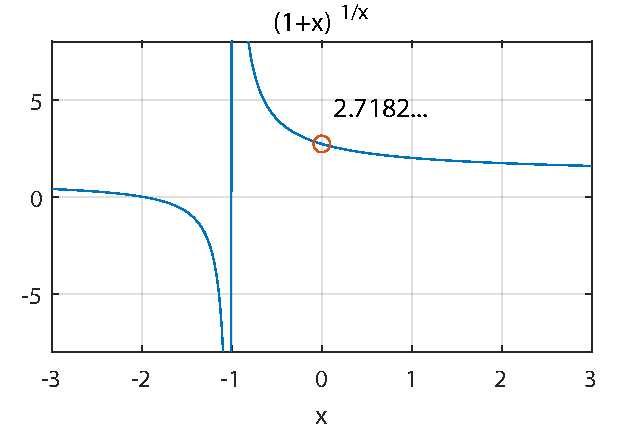
\includegraphics[width=8cm]{./figures/E_1.pdf}
\caption{$(1+x)^{1/x}$ 的函数图} \label{E_fig1}
\end{figure}

\autoref{E_tab1} 用数值计算验证\autoref{E_eq1} 的右极限.
\begin{table}[ht]
\centering
\caption{极限 $\E$ 数值验证(保留 6 位有效数字)}\label{E_tab1}
\begin{tabular}{|c|c|c|c|c|c|c|}
\hline
$x$ & $10^{-1}$ & $10^{-2}$ & $10^{-3}$ & $10^{-4}$ & $10^{-5}$ & $10^{-6}$ \\
\hline
$(1 + x)^{1/x}$ & $2.59374$ & $2.70481$ & $2.71692$ & $2.71815$ & $2.71827$ & $2.71828$ \\
\hline
\end{tabular}
\end{table}

\subsection{自然对数函数}
以 $\E$ 为底的对数函数 $\log_{\E} x$ 叫做\textbf{自然对数}, 通常记为
\begin{equation}
\ln x \qquad \text{或} \qquad \log x
\end{equation}
函数图如\autoref{E_fig2} .
\begin{figure}[ht]
\centering
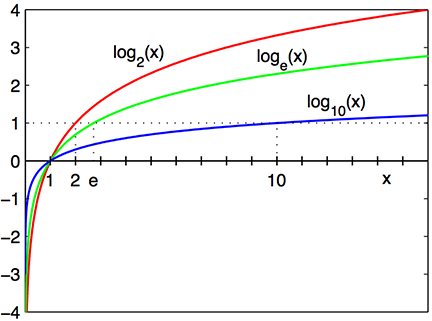
\includegraphics[width=7cm]{./figures/E_2.png}
\caption{几种不同底的对数函数} \label{E_fig2}
\end{figure}
